%%%%%%%%%%%%%%%%%%%%%%%%%%%%%%%%%
% baposter Landscape Poster
% LaTeX Template
% Version 1.0 (15/5/13)
%
% Created by:
% Brian Amberg (baposter@brian-amberg.de)
%
% This template has been downloaded from:
% http://www.LaTeXTemplates.com
%
% License:
% CC BY-NC-SA 3.0 (http://creativecommons.org/licenses/by-nc-sa/3.0/)
%
%%%%%%%%%%%%%%%%%%%%%%%%%%%%%%%%%%%%%%%%%

%----------------------------------------------------------------------------------------
%	PACKAGES AND OTHER DOCUMENT CONFIGURATIONS
%----------------------------------------------------------------------------------------

\documentclass[paperwidth=36in, paperheight=48in,portrait,fontscale=0.35, margin=2cm]{baposter}

\usepackage[utf8]{inputenc}
\usepackage[font=normalsize,labelfont=bf]{caption} % Required for specifying captions to tables and figures
\captionsetup{justification=centering}
\usepackage{booktabs} % Horizontal rules in tables
\usepackage{lmodern}
\usepackage{relsize} % Used for making text smaller in some places

% Other packages
\usepackage{tabularx}
\def\tabularxcolumn#1{m{#1}}
\def\imagetop#1{\vtop{\null\hbox{#1}}}
\usepackage{adjustbox}
\usepackage{subfig}
\usepackage{floatrow} % sidecapfloat
\usepackage{setspace}
\usepackage{xspace}
\usepackage{noReferences}
\usepackage{caption}
\usepackage{tikz}
\usepackage[customcolors]{hf-tikz}
%\usepackage{subcaption}
\usepackage{epsf}
\usepackage{amsmath}
\usepackage{mathtools}
\usepackage{amssymb}
\usepackage{amsfonts}
\usepackage{amsthm}
\usepackage{dsfont}
\usepackage{enumitem}
\usepackage{float}
\usepackage{cases}
\usepackage{verbatim}
\usepackage{array}
\usepackage{graphicx}
\usepackage{graphics}
\usepackage{multirow}
\usepackage{listings}
%\usepackage[authoryear]{natbib}
\usepackage{authblk}
\usepackage[linesnumbered,ruled,vlined]{algorithm2e}
\usepackage{eqparbox}
\usepackage{xcolor}
\usepackage[backend=biber, citestyle=authoryear, maxcitenames=2, maxbibnames=2]{biblatex}

\bibliography{../biblio.bib}


% Arrows
\newcommand{\incarrow}{{
\includegraphics[height=0.7\baselineskip]{./img/arrow_list}}}

% Colors for slides
\definecolor{rouge1}{RGB}{226,0,38}  % red P
\definecolor{orange1}{RGB}{243,154,38}  % orange P
\definecolor{jaune}{RGB}{254,205,27}  % jaune P
\definecolor{blanc}{RGB}{255,255,255} % blanc P

\definecolor{rouge2}{RGB}{230,68,57}  % red S
\definecolor{orange2}{RGB}{236,117,40}  % orange S
\definecolor{taupe}{RGB}{134,113,127} % taupe S
\definecolor{gris}{RGB}{91,94,111} % gris S
\definecolor{bleu1}{RGB}{38,109,131} % bleu S
\definecolor{bleu2}{RGB}{28,50,114} % bleu S
\definecolor{vert1}{RGB}{133,146,66} % vert S
\definecolor{vert3}{RGB}{20,200,66} % vert S
\definecolor{vert2}{RGB}{157,193,7} % vert S
\definecolor{vertsolarized}{RGB}{211,233,219} % vert S
\definecolor{darkyellow}{RGB}{233,165,0}  % orange S
\definecolor{lightgray}{rgb}{0.9,0.9,0.9}
\definecolor{darkgray}{rgb}{0.6,0.6,0.6}

% Highlights for slides
\newcommand{\rcol}[1]{\textcolor{red}{\textit{#1}}}
%\newcommand{\eqrcol}[1]{\textcolor{red}{#1}}
%\newcommand{\eqrcolb}[1]{\textcolor{red}{\boldsymbol{#1}}}
\newcommand{\gcol}[1]{\textcolor{vert3}{\textit{#1}}}
%\newcommand{\eqgcol}[1]{\textcolor{vert3}{#1}}
%\newcommand{\eqgcolb}[1]{\textcolor{vert3}{\boldsymbol{#1}}}
\newcommand{\blcol}[1]{\textcolor{blue}{\textit{#1}}}
%\newcommand{\eqbcol}[1]{\textcolor{blue}{#1}}
%\newcommand{\eqbcolb}[1]{\textcolor{blue}{\boldsymbol{#1}}}
\newcommand{\ycol}[1]{\textcolor{darkyellow}{\textit{#1}}}
\newcommand{\eqycol}[1]{\textcolor{darkyellow}{#1}}

\newcommand{\rcolbm}[1]{$\textcolor{red}{\boldsymbol{#1}}$}
\newcommand{\rcolb}[1]{\textcolor{red}{\textit{\textbf{#1}}}}
\newcommand{\gcolb}[1]{\textcolor{vert3}{\textit{\textbf{#1}}}}
\newcommand{\bcolb}[1]{\textcolor{blue}{\textit{\textbf{#1}}}}
\newcommand{\ycolb}[1]{\textcolor{darkyellow}{\textit{\textbf{#1}}}}

% Colored boxes
\newcounter{ColoredBoxesCounter}
\newcommand{\highlightnew}[3][(0.0,-0.1)(-0.0,0.3)]{
\hfsetfillcolor{#2!20}
\hfsetbordercolor{#2!80}
\tikzmarkin{\theColoredBoxesCounter}#1
#3
\tikzmarkend{\theColoredBoxesCounter}
\stepcounter{ColoredBoxesCounter}
}

\newcommand{\highlight}[2][yellow]{\mathchoice%
{\colorbox{#1}{$\displaystyle#2$}}%
{\colorbox{#1}{$\textstyle#2$}}%
{\colorbox{#1}{$\scriptstyle#2$}}%
{\colorbox{#1}{$\scriptscriptstyle#2$}}}%

\newcommand{\eqrcol}[1]{\highlight[red!20]{#1}}
\newcommand{\eqrcolb}[1]{\highlight[red!20]{\boldsymbol{#1}}}
\newcommand{\eqgcol}[1]{\highlight[vert3!20]{#1}}
\newcommand{\eqgcolb}[1]{\highlight[vert3!20]{\boldsymbol{#1}}}
\newcommand{\eqbcol}[1]{\highlight[blue!20]{#1}}
\newcommand{\eqbcolb}[1]{\highlight[blue!20]{\boldsymbol{#1}}}

\colorlet{redp}{red!20} % vert S
\colorlet{greenp}{vert3!20} % vert S
\colorlet{bluep}{blue!20} % vert S
\colorlet{yellowp}{yellow!20} % vert S

\newcommand{\hl}[3][\fboxsep1pt]{{#1\colorbox{#2}{#3}}}%

\newcommand{\hlr}[1]{\hl{redp}{#1}}
\newcommand{\hlg}[1]{\hl{greenp}{#1}}
\newcommand{\hlb}[1]{\hl{bluep}{#1}}
\newcommand{\hly}[1]{\hl{yellowp}{#1}}

\newcommand{\hler}[1]{\hl[\fboxsep0pt]{redp}{$\displaystyle {#1}$}}
\newcommand{\hleg}[1]{\hl[\fboxsep0pt]{greenp}{$\displaystyle {#1}$}}
\newcommand{\hleb}[1]{\hl[\fboxsep0pt]{bluep}{$\displaystyle {#1}$}}

\newcommand{\hlbr}[1]{\hl[\fboxsep0pt]{redp}{$\displaystyle \mathbf{#1}$}}
\newcommand{\hlbg}[1]{\hl[\fboxsep0pt]{greenp}{$\displaystyle \mathbf{#1}$}}
\newcommand{\hlbb}[1]{\hl[\fboxsep0pt]{bluep}{$\displaystyle \mathbf{#1}$}}

\newcommand{\vph}{\vphantom{A_A^A}}

% Box for algorithms
\newlength{\minipagewidth}
\newlength{\minipagewidthx}
\setlength{\minipagewidth}{\columnwidth}
\setlength{\minipagewidthx}{\columnwidth}
\setlength{\fboxsep}{0.1mm}
\addtolength{\minipagewidth}{-\fboxrule}
\addtolength{\minipagewidth}{-\fboxrule}
\addtolength{\minipagewidth}{-\fboxsep}
\addtolength{\minipagewidth}{-\fboxsep}
\addtolength{\minipagewidthx}{+\fboxsep}
\newcommand{\bookbox}[1]{\small
\par\medskip\noindent
\framebox[\columnwidth]{
\begin{minipage}{\minipagewidth} {#1} \end{minipage} } \par\medskip }

\newcommand{\bookboxx}[1]{
\par\medskip\noindent
\framebox[\columnwidth]{
\begin{minipage}[t]{0.98\columnwidth} {\par\smallskip#1\par\smallskip} \end{minipage} } \par\medskip }


\usepackage{array}
\newcolumntype{L}[1]{>{\raggedright\let\newline\\\arraybackslash\hspace{-3.1cm}}m{#1}}
\newcolumntype{C}[1]{>{\centering\let\newline\\\arraybackslash\hspace{135pt}}m{#1}}
\newcolumntype{R}[1]{>{\raggedleft\let\newline\\\arraybackslash\hspace{-10pt}}m{#1}}

\newenvironment{myfont}{\fontfamily{kurier}\selectfont}{\par}
\newenvironment{myfont2}{\fontfamily{epigrafica}\selectfont}{\par}

% Border color of content boxes
\definecolor{bordercol}{RGB}{0,0,0}  %black
% Background color for the header in the content boxes (left side)
\definecolor{headercol1}{RGB}{200,0,0}        %red:RGB {200,0,0} 
% Background color for the header in the content boxes (right side) 
\definecolor{headercol2}{rgb}{1.0,0.49,0.0}        %orange:rgb {1.0,0.49,0.0}
% Text color for the header text in the content boxes
\definecolor{headerfontcol}{rgb}{1,1,1}  %white
% Background color for the content in the boxes
\definecolor{boxcolor}{rgb}{1,1,1} 

\definecolor{lightblue}{rgb}{0.145,0.6666,1}

\newsavebox\CBox
\newcommand\hcancel[2][0.5pt]{%
  \ifmmode\sbox\CBox{$#2$}\else\sbox\CBox{#2}\fi%
  \makebox[0pt][l]{\usebox\CBox}%  
  \rule[0.3\ht\CBox-#1/2]{\wd\CBox}{#1}}

%%% miso
\newcommand{\eps}{\varepsilon}
\newcommand{\vareps}{\varepsilon}
\renewcommand{\epsilon}{\varepsilon}
\renewcommand{\hat}{\widehat}
\renewcommand{\tilde}{\widetilde}
\renewcommand{\bar}{\overline}

%\newcommand{\CommaBin}{\mathbin{\raisebox{0.5ex}{,}}}
\newcommand*{\MyDef}{\mathrm{\tiny def}}
\newcommand*{\eqdefU}{\ensuremath{\mathop{\overset{\MyDef}{=}}}}% Unscaled version
\newcommand*{\eqdef}{\mathop{\overset{\MyDef}{\resizebox{\widthof{\eqdefU}}{\heightof{=}}{=}}}}

%%%%%%%%%%%%%%%%%%%%%%%%%%%%
% Paper dependent stuff    %
%%%%%%%%%%%%%%%%%%%%%%%%%%%%

\newcommand{\interval}[1]{\square #1}
\newcommand{\imin}[1]{\underline{#1}}
\newcommand{\imax}[1]{\overline{#1}}

\newcommand{\olop}{\textsc{OLOP}\xspace}
\newcommand{\klolop}{\textsc{KL-OLOP}\xspace}



%%%%%%%%%%%%%%%%%%%%%%%%%%%%
% Aesthetics               %
% over-underline, hat, bold%
%%%%%%%%%%%%%%%%%%%%%%%%%%%%
\def\:#1{\protect \ifmmode {\mathbf{#1}} \else {\textbf{#1}} \fi}
\newcommand{\CommaBin}{\mathbin{\raisebox{0.5ex}{,}}}

\newcommand{\wt}[1]{\widetilde{#1}}
\newcommand{\wh}[1]{\widehat{#1}}
\newcommand{\wo}[1]{\overline{#1}}
\newcommand{\wb}[1]{\overline{#1}}

% bf and bm missing due to conflict!!
\newcommand{\bsym}[1]{\mathbf{#1}}
\newcommand{\bzero}{\mathbf{0}}
\newcommand{\ba}{\mathbf{a}}
\newcommand{\bb}{\mathbf{b}}
\newcommand{\bc}{\mathbf{c}}
\newcommand{\bd}{\mathbf{d}}
\newcommand{\be}{\mathbf{e}}
\newcommand{\bg}{\mathbf{g}}
\newcommand{\bh}{\mathbf{h}}
\newcommand{\bi}{\mathbf{i}}
\newcommand{\bj}{\mathbf{j}}
\newcommand{\bk}{\mathbf{k}}
\newcommand{\bl}{\mathbf{l}}
\newcommand{\bn}{\mathbf{n}}
\newcommand{\bo}{\mathbf{o}}
\newcommand{\bp}{\mathbf{p}}
\newcommand{\bq}{\mathbf{q}}
\newcommand{\br}{\mathbf{r}}
\newcommand{\bs}{\mathbf{s}}
\newcommand{\bt}{\mathbf{t}}
\newcommand{\bu}{\mathbf{u}}
\newcommand{\bv}{\mathbf{v}}
\newcommand{\bw}{\mathbf{w}}
\newcommand{\bx}{\mathbf{x}}
\newcommand{\by}{\mathbf{y}}
\newcommand{\bz}{\mathbf{z}}

\newcommand{\bA}{\mathbf{A}}
\newcommand{\bB}{\mathbf{B}}
\newcommand{\bC}{\mathbf{C}}
\newcommand{\bD}{\mathbf{D}}
\newcommand{\bE}{\mathbf{E}}
\newcommand{\bF}{\mathbf{F}}
\newcommand{\bG}{\mathbf{G}}
\newcommand{\bH}{\mathbf{H}}
\newcommand{\bI}{\mathbf{I}}
\newcommand{\bJ}{\mathbf{J}}
\newcommand{\bK}{\mathbf{K}}
\newcommand{\bL}{\mathbf{L}}
\newcommand{\bM}{\mathbf{M}}
\newcommand{\bN}{\mathbf{N}}
\newcommand{\bO}{\mathbf{O}}
\newcommand{\bP}{\mathbf{P}}
\newcommand{\bQ}{\mathbf{Q}}
\newcommand{\bR}{\mathbf{R}}
\newcommand{\bS}{\mathbf{S}}
\newcommand{\bT}{\mathbf{T}}
\newcommand{\bU}{\mathbf{U}}
\newcommand{\bV}{\mathbf{V}}
\newcommand{\bW}{\mathbf{W}}
\newcommand{\bX}{\mathbf{X}}
\newcommand{\bY}{\mathbf{Y}}
\newcommand{\bZ}{\mathbf{Z}}

%%%%%%%%%%%%%%%%%%%%%%%%%%%%
% Math jargon              %
%%%%%%%%%%%%%%%%%%%%%%%%%%%%
\newcommand{\wrt}{w.r.t.\xspace}
\newcommand{\defeq}{\stackrel{\mathclap{\normalfont\mbox{\tiny def}}}{=}}
\newcommand{\maxund}[1]{\max\limits_{#1}}
\newcommand{\minund}[1]{\min\limits_{#1}}
\renewcommand{\epsilon}{\varepsilon}
\newcommand{\bigotime}{\mathcal{O}}


\DeclareMathOperator*{\argmin}{arg\,min} 
\DeclareMathOperator*{\argmax}{arg\,max} 
\DeclareMathOperator*{\cupdot}{\mathbin{\mathaccent\cdot\cup}}
% \newcommand{\eqdef}{\buildrel \text{def}\over =}

%%%%%%%%%%%%%%%%%%%%%%%%%%%%
% Matrix operators         %
%%%%%%%%%%%%%%%%%%%%%%%%%%%%
\newcommand{\transpose}{^\mathsf{\scriptscriptstyle T}}
\newcommand{\transp}{\mathsf{\scriptscriptstyle T}}

%%%%%%%%%%%%%%%%%%%%%%%%%%%%
% Statistic operators      %
%%%%%%%%%%%%%%%%%%%%%%%%%%%%
\newcommand{\probability}{\mathbb{P}}
\newcommand{\probdist}{Pr}
\DeclareMathOperator*{\expectedvalue}{\mathbb{E}}
\DeclareMathOperator*{\variance}{\text{Var}}
\newcommand{\expectedvalueover}[1]{\expectedvalue\limits_{#1}}
\newcommand{\condbar}{\;\middle|\;}
\newcommand{\gaussdistr}{\mathcal{N}}
\newcommand{\uniformdistr}{\mathcal{U}}
\newcommand{\bernoullidist}{\mathcal{B}}

%%%%%%%%%%%%%%%%%%%%%%%%%%%%
% Algebraic Sets           %
%%%%%%%%%%%%%%%%%%%%%%%%%%%%
\newcommand{\Real}{\mathbb{R}}
\newcommand{\Natural}{\mathbb{N}}
\newcommand{\statespace}{\mathcal{X}}
\newcommand{\funcspace}{\mathcal{F}}
\newcommand{\dynaspace}{\mathcal{T}}


\newtheorem{theorem}{Theorem}
\newtheorem{definition}{Definition}
\newtheorem{lemma}{Lemma}
\newtheorem{proposition}{Proposition}
\newtheorem{assumption}{Assumption}
\newtheorem{remark}{Remark}
\newtheorem{property}{Property}





\begin{document}


%\background{ % Set the background to an image (background.pdf)
%\begin{tikzpicture}[remember picture,overlay]
%\draw (current page.north west)+(-2em,2em) node[anchor=north west]
%{\includegraphics[height=1.1\textheight]{background.png}};
%\end{tikzpicture}
%}
\begin{poster}{
grid=false,
borderColor=bordercol, % Border color of content boxes
headerColorOne=headercol1, % Background color for the header in the content boxes (left side)
headerColorTwo=headercol2, % Background color for the header in the content boxes (right side)
headerFontColor=headerfontcol, % Text color for the header text in the content boxes
boxColorOne=boxcolor, % Background color for the content in the content boxes
headershape=roundedright, % Specify the rounded corner in the content box headers
%headerfont=\Large\sf\bf, % Font modifiers for the text in the content box headers
headerfont=\Large\bf\textsc, %Sans Serif
textborder=rectangle,
background=none,
headerborder=open, % Change to closed for a line under the content box headers
boxshade=plain,
textfont={\setlength{\parindent}{0.0em}\sffamily},
headerheight={0.05\textheight},
eyecatcher=true
%columns=5
}
%
%----------------------------------------------------------------------------------------
%	Title and authors
%----------------------------------------------------------------------------------------
%
{

\includegraphics[width=14em]{./img/renault_group}
}
{
Approximate Robust Control of Uncertain\\Dynamical Systems
}
{
Edouard Leurent, Yann Blanco, Denis Efimov, Odalric-Ambrym Maillard
\vspace{-3\baselineskip}
}
{

\includegraphics[width=14em]{./img/inria_sc}
}

\setlength{\colheight}{0.92\textheight}

%----------------------------------------------------------------------------------------
%	Motivation
%----------------------------------------------------------------------------------------

\headerbox{\textsc{Motivation}}{name=motivation,span=1,column=0,row=0}{
\begin{center}
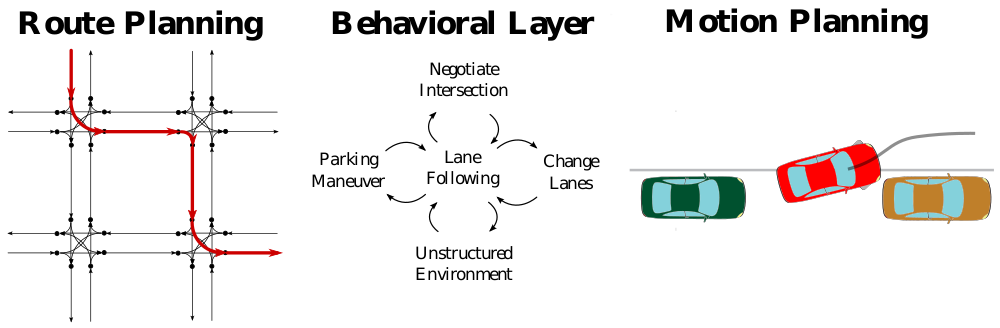
\includegraphics[width=\textwidth]{../img/pipeline}    
\textbf{Decision-making} pipeline in Autonomous Driving
\end{center}

\textbf{Progress has been made} {\small \parencite{Paden2016}}
\begin{itemize}[nolistsep]
\item[$\eqgcolb{\blacktriangleright}$] \hlg{route planning} is solved
\item[$\eqbcolb{\blacktriangleright}$] reliable techniques exist for \hlb{motion planning} and \hlb{control}
\end{itemize}

\vspace{.5\baselineskip}
\textbf{Current limitations}
\begin{itemize}[nolistsep,leftmargin=0.55cm]
\item[$\eqrcolb{\blacktriangleright}$] Implementations rely on \hlr{hand-crafted rules} such as FSM
\item[] \incarrow tailored for \hlr{specific} cases, won't \hlr{scale} to complex scenes
\item[$\eqrcolb{\blacktriangleright}$] Social interactions are difficult to model explicitly:
\item[] \incarrow poor \hlr{negotiation} abilities, \hlr{"freezing robot"} problem
\end{itemize}

\vspace{.5\baselineskip}
\textbf{We frame the problem in a sequential learning setting}
}

%----------------------------------------------------------------------------------------
%	Setting
%----------------------------------------------------------------------------------------
\headerbox{\textsc{Reinforcement learning}}{name=setting,span=1,column=0,row=0,below=motivation}{

    \hlb{\textbf{Optimal}} control under \hlr{unknown} dynamics $T(s_{t+1} | s_t, a_t)$

    \begin{equation}
        \max_\pi \expectedvalue \underbrace{\left[\sum_{t=0}^\infty \gamma^t r(s_t, a_t) \condbar \hleg{a_t\sim\pi(s_t)}, \hler{s_{t+1}\sim T(s_t, a_t)}\right]}_{\text{policy return }R^T_\pi}
    \end{equation}
    
    \textbf{Model-free} methods directly optimize $\hleg{\pi(a_t | s_t)}$ through policy evaluation and policy improvement.
    \vspace{1em}

    \textbf{Model-based} methods
    \begin{enumerate}[itemsep=0pt]
        \item Learn a model for the dynamics $\hler{\hat{T}(s_t, a_t)}$
        \item (Planning) Leverage it to compute
        \begin{equation*}
        \max_\pi \expectedvalue \left[\sum_{t=0}^\infty \gamma^t r(s_t, a_t) \condbar \hleg{a_t\sim\pi(s_t)}, \hler{s_{t+1}\sim \hat{T}(s_t, a_t)}\right]
        \end{equation*}
    \end{enumerate}


    \begin{itemize}[nolistsep]
        \item[$\eqgcolb{\blacktriangleright}$] Better \hlg{sample efficiency}, \hlg{interpretability}
        \item[$\eqrcolb{\blacktriangleright}$] $\hler{\text{Model bias: }\hat{T} \neq T}$
    \end{itemize}

}

%----------------------------------------------------------------------------------------
% Tools
%----------------------------------------------------------------------------------------
\headerbox{\textsc{Robust optimization}}
%{name=tools,column=2,span =2}
{name=tools,column=0,below=setting,span =1}
{
\begin{enumerate}[nolistsep]
    \item Build a \textbf{confidence region} $\bT$ around $\hler{T}$
    \begin{equation*}
    \forall T'\in \bT, \quad \probability(||\hler{T} - T'|| > \epsilon) < \delta
    \end{equation*}
    \item Plan \textbf{robustly} with respect to this ambiguity
    \begin{equation}
        \hleg{\max_{\pi}}\ \underbrace{\hler{\min_{T\in \bT}} \expectedvalue \sum_{t=0}^\infty \gamma^t r_t}_{v^r(\pi)} 
    \end{equation}
\end{enumerate}

\textbf{One-step} game between the planner and the environment:
\begin{itemize}[nolistsep]
    \item[1.] the \hlg{learner} reveals its policy $\hleg{\pi}$
    \item[2.] the \hlr{adversary} chooses the worst-case dynamics $T$
\end{itemize}

\begin{center}
    \hlb{\textbf{Assumption}}
\end{center}
We consider deterministic systems: $s_{t+1} = T(s_t, a_t)$

\begin{center}
\hlr{\textbf{Challenge}} 
\end{center}
How to optimize this objective?
\begin{itemize}[nolistsep]
    \item \hlg{Linear} system: $\mathcal{H}_\infty$ control, robust LQ
    \item \hlg{Finite} state-space: Robust Dynamic Programming
    \item \hlr{Non-linear continuous} system: ?
\end{itemize}

}


%----------------------------------------------------------------------------------------
%	Discrete Ambiguity
%----------------------------------------------------------------------------------------
\headerbox{\textsc{Discrete ambiguity and tree-based planning}}{name=discrete,column=1,span=2}{
\vspace{-.25\baselineskip}

\begin{center}
    \hlb{\textbf{Assumption}}
\end{center}
The ambiguity set $\bT$ and the action space $\mathcal{A}$ are discrete and \textbf{finite}: $
 \hleb{\bT = \{T_m\}_{m\in[1, M]}} \quad \text{and} \quad \mathcal{A} = \{a_k\}_{k\in[1, K]}$
 
 We propose a robust version of \textbf{optimistic planning} for deterministic systems {\small \parencite{Hren2008}}


\begin{tabular}{>{\centering}p{0.63\textwidth}>{\centering}p{0.32\textwidth}}
\begin{minipage}[]{0.63\textwidth}
\bookboxx{
\begin{definition}
Given node $i\in\mathcal{T}$, define

\textbf{The robust value:}
$$v^r_i \eqdef \hleg{\vphantom{\min_{m\in[1, M]}}\max_{\pi \in i\mathcal{A^\infty}}} \hler{\min_{m\in[1, M]}} R^{T_m}_\pi$$

\textbf{The robust u-value:}
$$u_i^r(n) \eqdef
\begin{cases}
\hler{\min_{m\in[1, M]}} \sum_{t=0}^{d-1} \gamma^t r_t &\text{if } i \in \mathcal{L}_n \text{ ;}\\
\hleg{\max_{a\in\mathcal{A}}}\ u_{ia}^r(n) & \text{if } i \in \mathcal{T}_n \setminus \mathcal{L}_n
\end{cases}$$

\textbf{The robust b-value:}
$$b_i^r(n) \eqdef
\begin{cases}
\hler{\min_{m\in[1, M]}} \sum_{t=0}^{d-1} \gamma^t r_t + \frac{\gamma^d}{1-\gamma} &\text{if } i \in \mathcal{L}_n \text{ ;}\\
\hleg{\max_{a\in\mathcal{A}}}\ b_{ia}^r(n) & \text{if } i \in \mathcal{T}_n \setminus \mathcal{L}_n 
\end{cases}$$
\end{definition}
}
            
\bookboxx{
\begin{remark}[Ordering of min and max]
Naive comparison of action values between the different models do not recover the robust policy
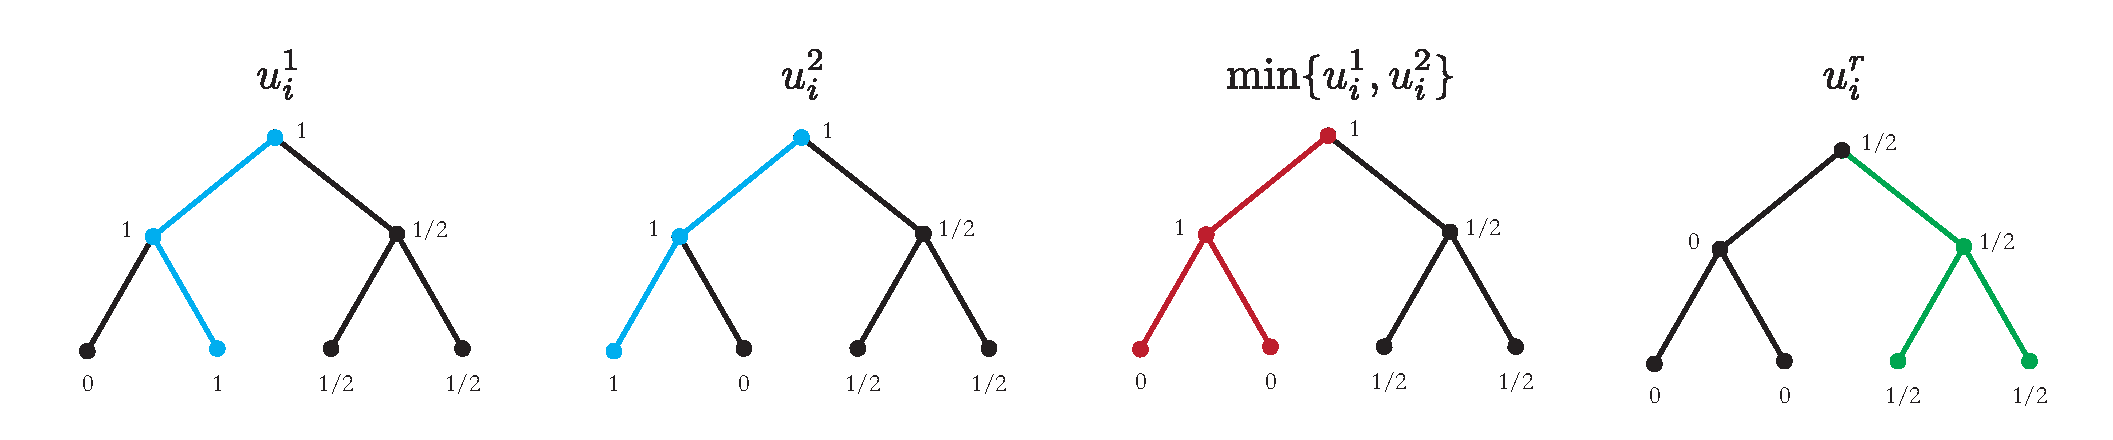
\includegraphics[width=\textwidth]{../img/min-max-order.eps}
\end{remark}
}
    
\bookboxx{
\begin{theorem}[Regret bound]
\label{theorem:drop-regret}
Algorithm \ref{algo:drop} enjoys a simple regret of:
\vspace{-0.5\baselineskip}
\begin{equation}
\text{If } \hler{\vph\kappa}>1,\qquad 
\hleb{\vph\mathcal{R}_n} = O\left(\hleg{\vph n}^{-\frac{\log 1/\gamma}{\log \hler{\vph\kappa}}}\right)
\end{equation}
\vspace{-\baselineskip}
\begin{equation}
\text{If }\hler{\vph\kappa}=1,\qquad
\hleb{\vph\mathcal{R}_n} = O\left(\gamma^{\frac{(1-\gamma)^\beta}{c}\hleg{\vph n}}\right)
\end{equation}
\vspace{-\baselineskip}
\end{theorem}
}
\end{minipage}

&

\begin{minipage}[]{0.32\textwidth}
\begin{center}
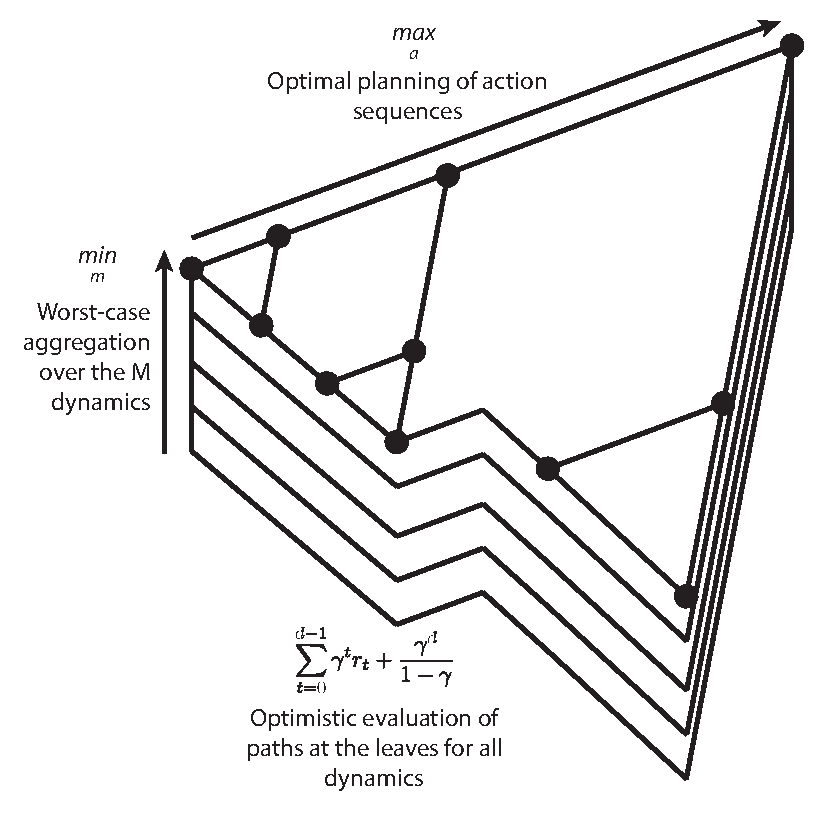
\includegraphics[width=.95\textwidth]{../img/robust-control-tree}    
\end{center}

\textbf{Variables}
\begin{itemize}[nolistsep]
    \item[\incarrow] computational \hlg{budget $n$}
    \item[\incarrow] near-optimal \hlr{branching factor $\kappa$}
    \item[\incarrow] simple regret \hlb{$\mathcal{R}_n = v^r - v^r_{a(n)}$}
\end{itemize}
\vspace{\baselineskip}
\begin{normalsize}
\begin{algorithm}[H]
\DontPrintSemicolon
Initialize $\mathcal{T}$ to a root and expand it. Set $n=1$.\;
\While{Numerical resource available}{
Compute the robust u-values $u^r_i(n)$ and robust b-values $b^r_i(n)$.\;
Expand $\argmax_{i\in \mathcal{L}_n} b^r_i(n)$.\;
n = n + 1\;
}
\Return $a(n) = \argmax_{a\in \mathcal{A}} u^r_a(n)$
\caption{Deterministic Robust Optimistic Planning}
\label{algo:drop}
\end{algorithm}
\end{normalsize}

\end{minipage}
\end{tabular}
}

%----------------------------------------------------------------------------------------
%	Continuous Ambiguity
%----------------------------------------------------------------------------------------
\headerbox{\textsc{Continuous ambiguity and interval-based planning}}{name=continuous,span=2,column=1,below=discrete}{ 

\begin{tabular}[T]{cc}
\begin{minipage}{0.49\textwidth}
\hlr{\textbf{Approximate}} the robust objective by a \hlg{tractable} surrogate. \vspace{-0.5\baselineskip}
\bookboxx{
\begin{definition} Given a policy $\pi$ and current state $s_0$, define
\textbf{The reachability set} $S$ at time $t$: 
$$S(t, s_0, \pi) \eqdef \{s_t: \exists T \in \bT \text{ s.t. } s_{k+1} = T(s_{k}, \pi(s_{k}))\}$$

\textbf{The interval hull} $\interval{S}=[\imin{s}, \imax{s}]$ {\small \parencite{Puig2005}}
$$\underline{s}(t, s_0, \pi) \eqdef \min S(t, s_0, \pi) \qquad \overline{s}(t, s_0, \pi) \eqdef \max S(t, s_0, \pi)$$
\end{definition}

\textbf{The surrogate objective} $\hat{v^r}$
\begin{equation}
\hleb{\vphantom{\frac{A}{A}}\hat{v^r}(\pi)} \eqdef \sum_{t=0}^H \gamma^t \min_{s\in \square S(t, s_0, \pi)}  r(s, \pi(s))
\end{equation}
}

The approximate performance of a policy is \hlg{guaranteed} on the true environment.
\vspace{-0.5\baselineskip}
\bookboxx{
\begin{proposition}[Lower bound]
\label{prop:lower-bound}
The surrogate objective $\hat{v^r}$ is a lower bound of the true objective $v^r$:

\begin{equation}
\forall \pi,\ \hleb{\vphantom{\frac{A}{A}}\hat{v^r}(\pi)} \leq \hler{\vphantom{\frac{A}{A}}v^r(\pi)}
\end{equation}
\end{proposition}
}

\end{minipage}

&

\begin{minipage}{0.47\textwidth}

\centering
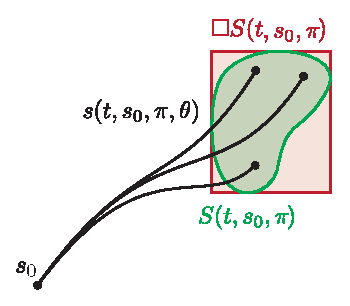
\includegraphics[width=0.7\textwidth]{../img/interval-hull}

\begin{footnotesize}
\begin{algorithm}[H]
  \SetAlgoLined\DontPrintSemicolon
  \SetKwFunction{algo}{robust\_control}\SetKwFunction{proc}{evaluate}
  \SetKwProg{myalg}{Algorithm}{}{}
  \myalg{\algo{$s_0$}}{
  Initialize a set $\Pi$ of policies\;
  \While{resources available}
  {
  \proc{} each policy $\pi\in\Pi$ at current state $s_0$\; 
  Update $\Pi$ by policy search\;  
  }
  \KwRet $\argmax_{\pi\in\Pi} \hleb{\hat{v^r}(\pi)}$ \;}{}
  \setcounter{AlgoLine}{0}
  \SetKwProg{myproc}{Procedure}{}{}
  \myproc{\proc{$\pi$, $s_0$}}{
  Compute the state interval $\interval{S}(t, s_0, \pi)$ on a horizon $t\in[0, H]$\;
  Minimize $r$ over the intervals $\interval{S}(t, s_0, \pi)$ for all $t\in[0, H]$\;
  \KwRet \hlb{$\hat{v^r}(\pi)$}\;}
\caption{Interval-based Robust Control}
\label{algo:irc}
\end{algorithm}
\end{footnotesize}
\end{minipage}
\end{tabular}

\vspace{.75\baselineskip}
}

%
%%----------------------------------------------------------------------------------------
%% Experiments
%%----------------------------------------------------------------------------------------
%
\headerbox{Experiments}{name=experiments,span=2,column=1,below=continuous, above=bottom}{ 

We introduce \textsc{highway-env}, a new environment for simulated highway driving and tactical decision-making\footnote{Video and source code are available at https://eleurent.github.io/robust-control/}.

In these experiments, the \hlg{ego-vehicle} is approaching a roundabout with
\hly{flowing traffic}. 

We first consider ambiguity with respect to the possible \hlr{destination} of each vehicle (fig \subref*{fig:destination}), and then \wrt their \hlr{driving style} (fig \subref*{fig:driving-style}).


\begin{figure}[H] 
  \centering 
  \begin{tabular}{l}
  \subfloat[Discrete ambiguity]{\adjustbox{raise=-3.6pc}{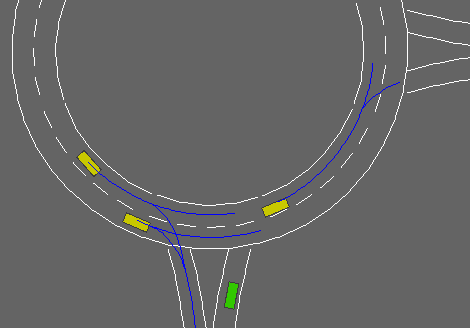
\includegraphics[width=0.27\textwidth]{../img/he-discrete.png}}\label{fig:destination}}\ 
  \subfloat[Continuous ambiguity]{\adjustbox{raise=-3.6pc}{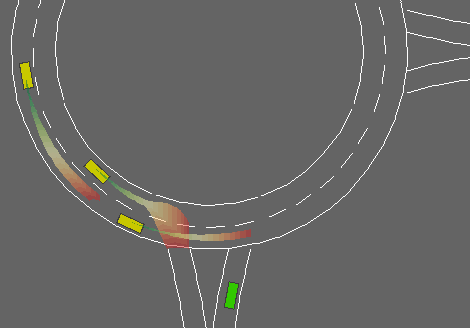
\includegraphics[width=0.27\textwidth]{../img/he-interval.png}\label{fig:driving-style}}}\
    \subfloat[Results]{
        \begin{tabular}{c c c c} \toprule
         Ambiguity & Agent & Worst-case & Mean $\pm$ std  \\ \midrule
         None & Oracle & $9.83$ & $10.84 \pm 0.16$ \\ \midrule
        \multirow{2}{*}{Discrete} & Nominal & $\hler{\vph 2.09}$ & $8.85 \pm 3.53$ \\
         & Algorithm \ref{algo:drop} & \textbf{$\hleg{\vph 8.99}$} &  \textbf{$10.78 \pm 0.34$} \\ \midrule
        \multirow{2}{*}{Continuous} & Nominal & $\hler{\vph 1.99}$ & $9.95 \pm 2.38$ \\
         & Algorithm \ref{algo:irc} & \textbf{$\hleg{\vph 7.88}$} & \textbf{$10.73 \pm 0.61$} \\ \bottomrule
         \end{tabular}
      }
  \end{tabular}
\end{figure}
}


%----------------------------------------------------------------------------------------
%	Acknowledgements
%----------------------------------------------------------------------------------------
\headerbox{Acknowledgements}{name=ack,column=0,span=1,below=tools}{
This work has been supported by CPER Nord-Pas de Calais/FEDER DATA Advanced data science and technologies 2015-2020, the French Ministry of Higher Education and Research, INRIA, and the French Agence Nationale de la Recherche (ANR).
}


%----------------------------------------------------------------------------------------
%	References
%----------------------------------------------------------------------------------------
\headerbox{References}{name=refs,column=0,span=1,below=ack, above=bottom}{
    {
    \AtNextBibliography{\footnotesize}
    \setlength{\bibitemsep}{3pt}
    \printbibliography[heading=none]
    }
}


\end{poster}

\end{document}


